\subsection{Intégration avec PHP et Laravel}% (fold)
\label{sub:integration_avec_php_et_laravel}

	MongoDB bénéficie d'une extension PHP facilement installable via PEAR (le gestionnaire d'extensions de PHP). Deux limitations existent néanmoins : le support de la version 3.0 de MongoDB n'est pas encore pris en charge et l'extension n'est pas encore compatible avec la toute dernière version majeure de PHP (PHP 7.0) prévue pour fin novembre. La mise à jour de l'extension vers la toute dernière version de MongoDB et de PHP sera sans doute effective rapidement.\\

	Afin de faciliter le développement, il a été décidé d'utiliser un ORM. Dans le cas des bases de données orientées documents, nous allons utiliser un ODM pour Object Document Mapping. Plusieurs grands ORM existent dans le monde des frameworks PHP : Doctrine et Eloquent sont deux des plus connus. Tous deux proposent un ODM associé. Doctrine présente l'avantage de permettre une intégration de MongoDB via un package PHP officiel. Eloquent supporte le système de base de données MongoDB via un package non-officiel (développé par jenssegers) appelé tout simplement \verb|mongodb|. Dans les deux cas, l'outil permet de gérer toutes les opérations de base ainsi que les documents imbriqués. Nous avons décidé d'utiliser Laravel et donc son ORM officiel Eloquent, nous allons donc utiliser le package \verb|jenssegers/mongodb| dans sa version 2.0.\\

	L'utilisation d'une base de données NoSQL est souvent délicate car il en existe de nombreux types différents et les intégrations ne sont donc pas forcément toutes développées (et rarement intégrée par des packages officiels). Il est donc préférable de se limiter aux bases de données les plus utilisées pour chaque type (MongoDB pour les bases de données orientées documents, Redis pour les bases de données orientées clé / valeur par exemple.). Dans notre cas, MongoDB étant très utilisée, il existe donc de nombreuses intégrations, comme nous l'avons vu pour PHP, mais aussi pour les différents ORM du marché ainsi que pour la plupart des solutions de test de l'écosystème (nous ne détaillerons pas les solutions de test dans ce rapport).

% subsection integration_avec_php_et_laravel (end)

\section{Modélisation de la base de données orientée documents}% (fold)
\label{sec:modelisation}

	Comme expliqué dans notre introduction aux bases de données orientées documents, il n'existe pas de schéma fixe pour ces dernières. Pour autant, lors du développement d'une vraie application, il est nécessaire pour les développeurs de se fixer des schémas afin de pouvoir utiliser la base de données.\\

	Nous avons organisé notre base de données en 4 collections : \verb|recipes|, \verb|locations|, \verb|guests| et \verb|events|.

	\subsection{Diagramme de stockage}

		\begin{figure}[H]
			\centering
			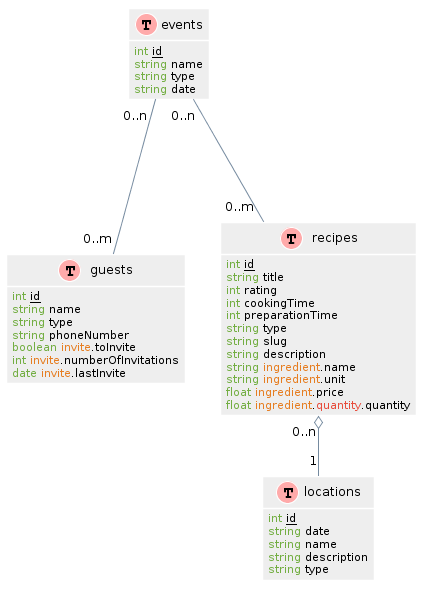
\includegraphics[width=0.5\textwidth]{images/diagramme-stockage.png}
			\caption{Diagramme de stockage de l'application dans une base de données orientée documents.}
			\label{fig:diagramme-stockage}
		\end{figure}

		Le diagramme de stockage de notre application est présenté dans la figure~\ref{fig:diagramme-stockage}. Les clés primaires de chaque collection sont soulignées. Les documents imbriqués sont représentés par des variations de couleurs dans les champs d'une collection. Les champs supplémentaires nécessaires aux relations \enquote{plusieurs vers plusieurs} ne sont pas représentés.

	\subsection{Recettes et ingrédients}

		Les recettes sont stockées dans la collection \verb|recipes|. Il n'existe pas de collection pour les ingrédients et leur quantité associée car nous avons décidé d'utiliser l'imbrication de documents afin de les stocker directement dans chaque recette.

		\paragraph{Avantage de la solution}% (fold)
			Lors de la récupération de chaque recette, les ingrédients sont automatiquement récupérés. Nous savons que dans la majorité des cas les informations sur les ingrédients seront nécessaire à l'affichage d'une recette, cette solution présente donc un avantage au niveau des performances (un seul document est à récupérer pour afficher une recette avec ses ingrédients). De plus, dans le cas présent, les ingrédients sont très succints (nom, unité, quantité et prix) et chaque recette ne possède que peu d'ingrédients donc cette solution ne va pas surcharger notre document parent.
		% paragraph avantage_de_la_solution (end)

		\paragraph{Désavantage de la solution}% (fold)
			Avec cette approche, il est très coûteux de récupérer la liste de tous les ingrédients car il faut parcourir toutes les recettes. De plus, cette solution nous oblige à dupliquer des informations pour chaque recette ayant des ingrédients identiques. Mettre à jour un ingrédient spécifique nous obligera à modifier indépendamment chaque recette utilisant cet ingrédient.
		% paragraph desavantage_de_la_solution (end)

		\paragraph{Avantages contre désavantages}% (fold)
			Dans notre application, le cas d'utilisation le plus utilisé sera l'affichage de recette. Il est donc préférable d'optimiser les lectures via l'imbrication. La possibilité de mettre à jour les ingrédients n'est pas prévue et dans le cas où elle serait ajoutée, elle resterait très rare par rapport à l'affichage. Le coût de mise à jour n'est donc pas un problème.
		% paragraph avantages_contre_desavantages (end)

	\subsection{Localisations}

		Les localisations sont stockées dans la collection \verb|locations|. Pour les localisations, trois choix sont possibles : stocker les localisations directement dans les documents \verb|recipe|, stocker les recettes dans les documents \verb|location| ou encore sotcker les documents \verb|recipe| et \verb|location| de manière indépendante et les lier via une clé étrangère.

		\paragraph{Avantage du stockage dans le document recipe}% (fold)
			Cette méthode de stockage permet d'améliorer les performances lors de l'affichage d'une recette. Cas d'utilisation très courant.
		% paragraph avantage_de_la_solution (end)

		\paragraph{Désavantage du stockage dans le document recipe}% (fold)
			Cette méthode complexifie le traitement des recettes via leur localisations. Il est plus coûteux d'afficher toutes les requettes d'une localisation par exemple.
		% paragraph desavantage_de_la_solution (end)

		\paragraph{Avantage du stockage dans le document location}% (fold)
			Cette méthode de stockage permet d'améliorer les performances lors de l'affichage d'une localisation avec toutes ses recettes.
		% paragraph avantage_de_la_solution (end)

		\paragraph{Désavantage du stockage dans le document location}% (fold)
			Les documents \verb|location| peuvent devenir très importants (très grande taille) si de nombreuses recettes sont stockées au même endroit.
		% paragraph desavantage_de_la_solution (end)

		\paragraph{Avantage du stockage séparé}% (fold)
			Cette méthode permet de gérer les recettes et les localisations de manière indépendante. Cette méthode est aussi la plus simple au niveau de la modélisation.
		% paragraph avantage_de_la_solution (end)

		\paragraph{Désavantage du stockage séparé}% (fold)
			Les requêtes ne sont pas optimisées dans les deux cas car MongoDB doit effectuer deux requêtes pour afficher une recette et $(n+1)$ requêtes pour afficher une localisation avec ses recettes.
		% paragraph desavantage_de_la_solution (end)

		\paragraph{Conclusion}% (fold)
			Nous avons décidé de gérer les recettes et les localisations de manière indépendante afin de simplifier la modélisation. Cette solution n'est pas parfaite et il faudrait savoir si il est préférable d'améliorer l'affichage des recettes ou celle des localisations ainsi que le nombre de recettes maximal pour une localisation (afin de savoir la taille probable de nos documents \verb|location|). Ce problème illustre les difficultés de modéliser une base de données lorsque les cas d'usages ne sont pas parfaitement connus.
		% paragraph conclusion (end)

		\paragraph{Solution alternative}% (fold)
			Il est également possible de combiner les deux stockages en dupliquant les informations. Par exemple, stocker dans le document \verb|recipe| sa localisation et stocker dans les documents \verb|location| un sous-ensemble (la recette sans ses ingrédients par exemple) de recette afin de limiter la taille. Cette solution présente les avantages des deux types de stockages et évite les requêtes multiples au détriment de la simplicité de la modélisation et des mises à jour des documents.
		% paragraph solution_alternative (end)

	\subsection{Invités}

		Les invités sont stockées dans la collection \verb|guests|. Cette collection est très simple car elle ne stocke qu'une seule entité. L'utilisation de MongoDB dans ce cas est la même que pour une base de données relationnelle.

	\subsection{Évènements}

		Les évènements sont stockées dans la collection \verb|events|. Tout comme pour les invités, cette collection est très simple car elle ne stocke qu'une seule entité.

	\subsection{Relations plusieurs à plusieurs}

		Il existe entre les invités et les évènements et entre les recette et les évènements des relations de plusieurs à plusieurs. En relationnel, ces relations sont gérés par une table de pivot contenant deux clés étrangères avec les identifiants de chaque modèle et optionnellement des caractéristiques de la relation. Les table pivot ne sont pas du tout optimisées pour les bases de données orientées documents. En effet, avec ces dernières, il est nécessaire d'effectuer une requête supplémentaire afin de récupérer le document correspondant à la relation. Toujours dans l'optique d'optimiser les lectures, notre ODM nous propose de gérer les relations plusieurs à plusieurs grâce à un tableau d'identifiant à la place d'une collection pivot. Il existe donc dans le document \verb|event| par exemple, deux tableaux d'identifiants : \verb|guest_ids| et \verb|recipe_ids|. Ces tableaux sont répétés dans le document \verb|guest| et dans le document \verb|recipe| avec un tableau \verb|event_ids|.

		\paragraph{Avantage de la solution}% (fold)
			À partir du moment où le document \verb|event| est récupéré, il est possible d'effectuer directement une nouvelle requête afin de récupérer les recettes ou les invités associés sans passer par une requête supplémentaire sur une collection pivot.
		% paragraph avantage_de_la_solution (end)

		\paragraph{Désavantage de la solution}% (fold)
			L'ajout ou la suppression d'une relation entre deux documents passent par la mise à jour des deux documents et non pas par l'insertion ou la suppression d'un document pivot unique.
		% paragraph desavantage_de_la_solution (end)

	\subsection{La vue AInviter}

		Dans le cadre du projet de base de données, il a été demandé de faciliter l'accès aux personnes à inviter en créant une vue des invités avec si oui ou non ils ont déjà été invité, le nombre d'évènements auquels ils ont participés et la date de la dernière invitation si cette dernière à eu lieu.\\

		Le système de vue n'existant pas dans les bases de données orientées document, nous avons créé un faux modèle imbriqué (un booléen indiquant si la personne a déjà été invité, le nombre d'invitation reçu par cette personne et la date de la dernière invitation) dans les invités afin de stocker ces informations dupliquées. Ce stockage sous forme de document imbriqué va améliorer les performances de lecture mais déteriorer les performances en écriture. En effet, à chaque nouvelle invitation d'un invité, il est nécessaire de mettre à jour ce document imbriqué avec les nouvelles valeurs.

% section modelisation (end)

\section{Utilisation d'une base de données clé-valeur}
	\subsection{Le besoin d'utiliser une base de données clé-valeur }
		Nous avons vu dans la sous-section précédente \ref{par:desavantage_de_la_solution} qu'il était très coûteux de récupérer la liste de tous les ingrédients. Pourtant cette opération doit être effectuée lors de l'ajout d'une recette. En effet, lors de l'ajout de la recette, il est nécessaire de choisir quels ingrédients sont nécessaires à la réalisation de la recette.\\

		Pour aider l'utilisateur, il est utile de lui suggérer les ingrédients déjà connus de l'application, lorsque celui-ci ajoute les ingrédients nécessaires à sa nouvelle recette. Il apparaît comme inenvisageable de devoir parcourir toutes les recettes, extraire tous les ingrédients de chaque recette et construire une liste d'ingrédients sans duplicatas pour répondre à ce cas d'utilisation.\\

		C'est lors de problématiques comme celles-ci qu'une base de données clé-valeur est utile. Une base de données clé-valeur peut permettre de stocker une valeur, issue d'un calcul coûteux, pendant une courte période.

	\subsection{Stockage de la liste des ingrédients}
		\subsubsection{Problème rencontré}
			L'idée principale est d'avoir accès facilement à une liste de tous les ingrédients. En réfléchissant un petit peu plus longtemps, on se rend compte qu'il pourrait être utile d'avoir des informations supplémentaires comme le prix et l'unité de la quantité associée à l'ingrédient. Le problème est que le prix d'un ingrédient n'est pas toujours le même, et l'unité de la quantité associée à l'ingrédient peut varier selon les goûts de chacun.\\

		\subsubsection{Solution retenue}
			Pour autant, l'utilisateur appréciera de se voir proposer des valeurs par défaut cohérentes lorsque celui-ci ajoutera un ingrédient déjà connu de l'application à une recette créée. On décide alors de définir le prix de l'ingrédient comme la moyenne des prix indiqués pour le même ingrédient (utilisé dans les autres recettes) et de fixer l'unité de la quantité associée à l'ingrédient comme celle la plus souvent choisie par les utilisateurs.\\

			Lors de l'ajout d'un ingrédient à une recette, si cet ingrédient n'existait pas encore, l'ingrédient est rajouté à la liste des ingrédients en base de données clé-valeur, avec son prix et l'unité de la quantité choisie. Si l'ingrédient existait déjà, le prix est mis à jour en calculant une nouvelle moyenne et l'unité de la quantité associée reste inchangée. La clé a un temps d'expiration de 30 minutes, ce qui veut dire que la liste des ingrédients avec la moyenne des prix et les unités sera automatiquement régénérée 30 minutes après la création de la clé. On trouve ici un bon compromis : un accès quasi instantané à une information coûteuse à calculer et la garantie de la quasi cohérence de cette information.\\

			Au final on obtient un grand gain de performance au prix de quelques lignes de code à écrire en plus et d'une base de données clé-valeur légère à déployer.
